\chapter{\ExaHyPE}
\label{section:exahype}


% \begin{figure}[htb]
 \begin{center}
  
\includegraphics[width=0.16\textwidth]{60_exahype/EU.png}
  
\includegraphics[width=0.35\textwidth]{60_exahype/ExaHyPE_Logo.jpg}
  
\includegraphics[width=0.27\textwidth]{60_exahype/ExCALIBUR.png}
 \end{center}
%  \caption{
 { \footnotesize
   The original ExaHyPE project delivering the first generation of the ExaHyPE
   software has received funding from the European Union’s Horizon 2020 research
   and innovation programme under grant agreement No 671698 (ExaHyPE).
   \ExaHyPE\ has been made possible by EPSRC under the grant EP/V00154X/1
   (ExaClaw). 
 }
% \end{figure}


\ExaHyPE\ is both a set of C/C++ and Fortran core routines complementing the
\Peano\ core and a high-level augmentation of \Peano's Python API.
\ExaHyPE's Python API can be read as builder mechanism:
You configure your particular \ExaHyPE\ application, i.e.~you tell the \ExaHyPE\
engine which application you want to run (which PDE terms, which solver
variants, which hardware properties).
The Python API then yields both a \Peano\ Python project which you can run plus
a set of template classes which you implement with your particular application.


The present document discusses how to create an \ExaHyPE\ application from
scratch.
Most application experts might not want to do this and instead use a read-to-use
\ExaHyPE\ application.
The most prominent (and maybe powerful) code using the ExaHyPE engine is maybe
ExaSeis; used to simulate seismic waves.
The details of these domain-specific codes are not covered by the present
document.


\begin{framed}
\paragraph*{First \ExaHyPE\ run}
\begin{itemize}
  \item Configure \Peano\ with the flags \texttt{--enable-exahype}
  \texttt{--enable-loadbalancing}:
  \begin{code}
libtoolize; aclocal; autoconf; autoheader; cp src/config.h.in .; automake --add-missing
./configure --enable-exahype --enable-loadbalancing
  \end{code}
   These are the two mandatory extensions. You might want to add further options.
  \item Recompile your \Peano\ code. This should give you a couple of
  \texttt{ExaHyPE2Core} libraries in the respective subdirectories.
  \item Ensure that \texttt{python} subdirectory is in your Python search path
  and
  \item run the Jupyter notebook in \texttt{examples/exahype2/euler}: 
  \begin{code}
export PYTHONPATH=../../../python/
jupyter-notebook Euler.ipynb
  \end{code}
  \noindent
  or---if you don't like Jupyter notebooks---type in
  \begin{code}
export PYTHONPATH=../../../python/
python3 example-scripts/finitevolumes-with-ExaHyPE2-benchmark.py --h 0.1
./peano4
  \end{code}
\end{itemize}
\end{framed}



\section{Historical remarks}

\ExaHyPE\ is the follow-up development of the ExaHyPE project which has
been funded by the EU from 2015--2019.
The present version is the second generation of the code (\ExaHyPE) and has
seen substantial rewrites of core routines.
However, many paradigms and even code blocks remain the same.
Migrating from the original ExaHyPE to \ExaHyPE\ thus should be straightforward.


The original ExaHyPE had been built on top of Peano (third generation) and tried
to hide as much of Peano away as possible.
In \ExaHyPE, I go the opposite way: \ExaHyPE\ is a full-blown Peano add-in and I
try not to hide anything away.
Where we designed our own data management on top of Peano in ExaHyPE, all the
data management (as well as parallelisation, e.g.) is native \Peano.


With the migration from a sole-C++ philosophy to C++ supplemented by a Python
API in \Peano, I also dumped ExaHyPE's former configuration/specification file
pradigma.
An \ExaHyPE\ application now is championed by a sole Python script.
This Python script yields a native \Peano\ application (builder mechanism) which
then assembles the application.



\section{Minimalist Finite Volumes for the Euler equations}
\label{section:exahype:fv}


\begin{remark}
 In the \texttt{examples/exahype2} directory, there are multiple \ExaHyPE\
 experiments. An \ExaHyPE\ project is mainly a Python script supplemented by
 some C++ user code. I offer most of these scripts as Jupyter notebook, but some
 also are available as plain Python scripts. If you prefer to run the Jupyter
 notebooks without the GUI, use \texttt{ipython3}.
\end{remark}


\noindent
A minimalist \ExaHyPE\ solver resembles:
\begin{code}
project = exahype2.Project( ["examples", "exahype2", "euler"], "finitevolumes", ".", "myexecname" )

project.add_solver(  exahype2.solvers.fv.GenericRusanovFixedTimeStepSizeWithEnclaves(
  "Euler",
  patch_size,
  unknowns, 0,
  min_h, max_h,
  time_step_size,
  flux = exahype2.solvers.fv.PDETerms.User_Defined_Implementation
))

project.set_global_simulation_parameters(
  dimensions, [0.0,0.0,0.0], [1.0,1.0,1.0],
  time_step_size * args.timesteps, # end time
  0.0, 0                           # snapshots
)

project.set_Peano4_installation( args.peanodir, build_mode )
peano4_project = project.generate_Peano4_project()
peano4_project.generate()
\end{code}

\begin{enumerate}
  \item We first create a new project. This is an \ExaHyPE\ project which is,
  for the time being, completely independent of a \Peano\ project.
  \item We next create a solver. 
  There's a number of solvers currently available within \ExaHyPE.
  Once created, we add it to the \ExaHyPE\ project before 
  \item we set the global simulation parameters.
  \item As \Peano\ has already been installed on the system, the developer did
  set all pathes, all compilers, all libraries, \ldots It would be inconvenient
  to ask a user to provide this information all over again. Therefore, we parse
  the outcome of \texttt{configure} and copy the relevant information over.
  \item Finally, we ask the \ExaHyPE\ project to generate a new \Peano\ project. 
\end{enumerate}


\noindent
Once we have a \Peano\ project, we can add further features to this one.
Eventually, we make the \Peano\ project generate the actual C++ code.


\paragraph{Created code.}
The above snippet does set up a complete \ExaHyPE\ simulation.
The solver will consist of two classes: \texttt{AbstractEuler} and a subclass
\texttt{Euler}.
The \texttt{Euler} is an empty stub when you call the script the first time.
You will have to befill it with the actual Physics---flux functions for example.
See the files in the directory \texttt{examples/exahype2/euler} which hosts such
example code. 
If you want to avoid to write C++ code at all, you can also use some symbolic
Python interface. 
An example for this one is provided via the Jupyter notebook.


\paragraph{Changing simulation properties.}
\ExaHyPE's Python API is written as end-to-end interface:
Whenever you change something, you have to run the whole script or Jupyter
notebook all over again.
In practice, this might be too much. 
Often, it is simply sufficient to repeat the following steps:

\begin{itemize}
  \item Change something within your \ExaHyPE\ project (such as the simulation
  runtime, or mesh size, or \ldots).
  \item Regenerate the resulting \Peano\ project: 
  \begin{code}
peano4_project = project.generate_Peano4_project()
  \end{code}
  \item Re-add all the stuff you had added to the \Peano\ project before,
  i.e.~additional libraries, additional compile flags, additional
  Fortran modules, \ldots Also set all the constants within the \Peano\ project
  that have to be exported into C++ code.
  \item Regenerate the C++ code:
  \begin{code}
peano4_project.generate( throw_away_data_after_generation=False )  
  \end{code}
\end{itemize}



\section{IO, logging and initialisation}


\ExaHyPE\ codes by default yield snapshots in \Peano's block format. 
That is, there's no distinguished \ExaHyPE\ format. 
Logging/state data is piped to the terminal or a file. 
It depends whether you have compiled \Peano\ with a special toolchain.


\paragraph{Patch file output}

The format as well as the postprocessing of \Peano's patch-file output is
discussed in Chapter \ref{chapter:postprocessing}.
By default, \ExaHyPE\ dumps all data as one large vector \texttt{Q} per Finite
Volume/integration point, i.e.~you get a set of scalars.
It also dumps all the resolution levels of the grid simultaneously.
Therefore, one of the first postprocessing steps usually is to remove all data
from the output data set besides the fine grid level.


\begin{remark}
 In principle, \Peano\ follows the philosophy that postprocessing should be done
 by postprocessing tools. It therefore just dumps the data (though efficiently
 in a bespoke format). For many applications, each dump of the whole
 simulation data is already too heavy. Therefore, you can add filters.
\end{remark}

\noindent
Filters can be added to your setup via
\begin{code}
probe_point = [0,0.693,0]
project.add_plot_filter( probe_point,[0.0,0.0,0.0],1 )
project.add_plot_filter( offset,size,10 )
\end{code}

\noindent
The example above sets a probe, i.e.~every plot step only the patch data around
the probe is dumped. Every 10 snapshot steps however, the whole domain is
written.
I assume that \texttt{offset} and \texttt{size} are configured accordingly.


The command
\begin{code}
project.set_output_path( "/scratch/myfolder" )
\end{code}
\noindent
configures \Peano\ with a proper output path. Without this command, all output
data is written to the working path.


\paragraph{Logging output}

\ExaHyPE\ searches for a text file \texttt{exahype.log-filter} in the working
directory.
If no such file is found (or the file is corrupted), then it will use some
default filter rules, i.e.~dump the information to the terminal that I consider
to be most important.
If you want to adopt the output, I strongly recommend that you add a log filter
configuration file. 


Often, users are only interested in a particular phase of the simulation or want 
to specify different log entries per program phase. The program phases offered
by default are
\begin{itemize}
  \item \texttt{create-grid-but-postpone-refinement}
  \item \texttt{create-grid}
  \item \texttt{create-grid-and-converge-load-balancing}
  \item \texttt{init-grid}
  \item \texttt{plot-solution}
  \item \texttt{time-step}
\end{itemize}

\noindent
The syntax of log filter files is discussed in Section
\ref{section:logging:log-filter}.


\paragraph{Solver initialisation}

If you have a complex solver setup, you might want to run some complex
initialisation at startup.
However, important parts of the \ExaHyPE\ infrastructure might not be up yet
when the solver's constructor is invoked.
So it is generally not a good idea to add too much setup routines to the
constructor.


Each solver has eight further routines that are of interest to squeeze in any
initialisation or global state update:

\begin{itemize}
  \item startGridConstructionStep
  \item finishGridConstructionStep
  \item startGridInitialisationStep
  \item finishGridInitialisationStep
  \item startTimeStep
  \item finishTimeStep
  \item startPlottingStep
  \item finishPlottingStep   
\end{itemize}


\noindent
If you plug into these, please ensure you continue to call the original
(superclass) routine still.
A typical pattern we've seen is to run some initialisation just prior to the
first grid construction step:

\begin{code}
class MyClass ... {
  void startGridConstructionStep() override;
  ...
};
\end{code}



\begin{code}
void MyClass::startGridConstructionStep() {
  // call superclass routine
  AbstractMyClass::startGridConstructionStep();
  static bool isInitialised = false;
  if (not isInitialised) {
    isInitialised = true;
    // your initialisation
  }
};
\end{code}

\section{Running on a parallel computer}

To run \ExaHyPE\ in parallel, you have to build \Peano\ with support for
multithreading and/or MPI.
Once this is done, the engine more or less runs in parallel out of the box.


\paragraph{Domain decomposition}
The core domain decomposition scheme realised in \ExaHyPE\ is a non-overlapping
multiscale domain decomposition based upon space-filling curves (SFC).
To use this scheme, you have to specify an appropriate load balancing scheme.
Without any load balancing, the code will never split up the domain and thus
effectively run serially.

\begin{figure}
 \begin{center}
  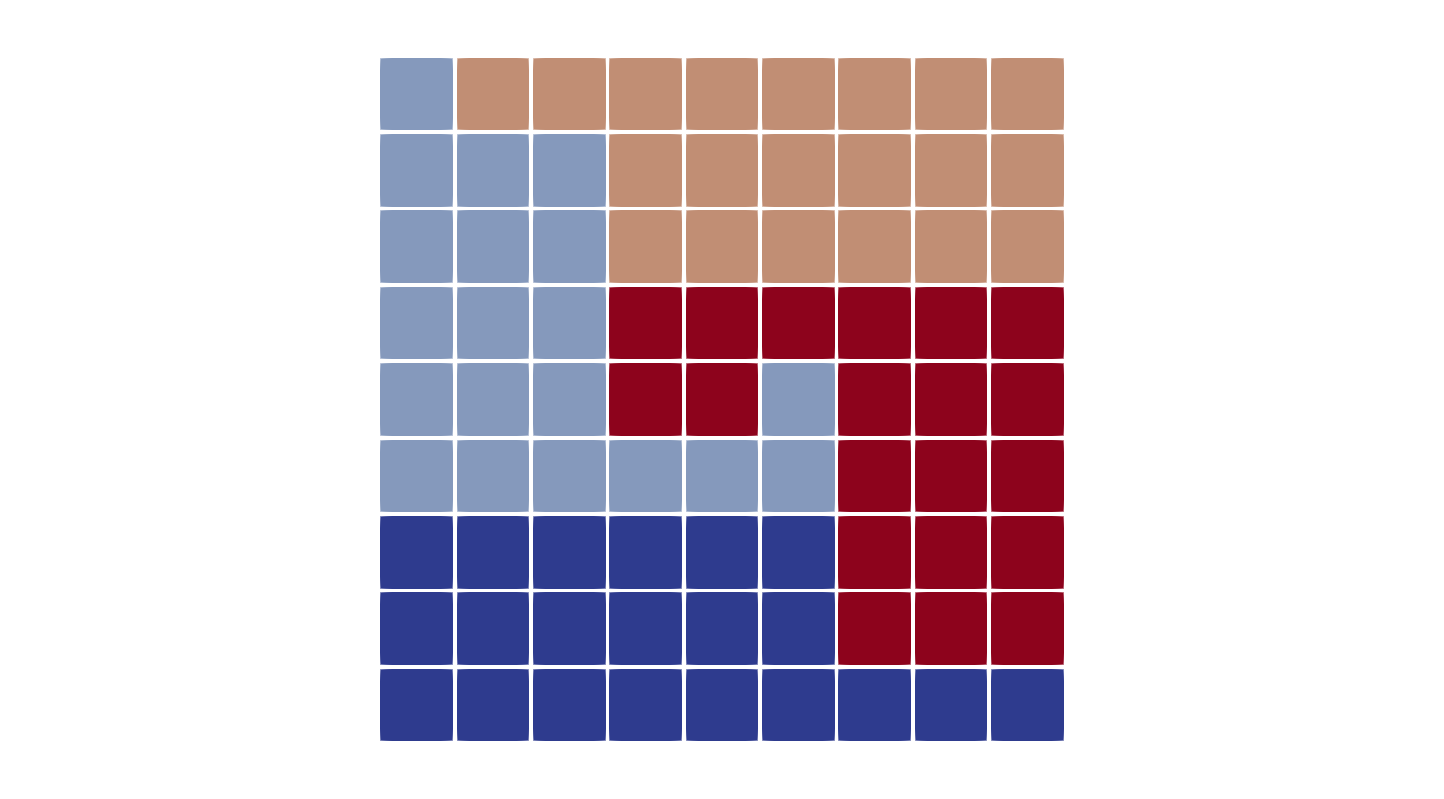
\includegraphics[width=0.54\textwidth]{60_exahype/domain-decomposition.png}
 \end{center}
 \caption{
  Domain decomposition in \ExaHyPE\ for a run with four threads/ranks. Each
  individual cell hosts a patch.
 }
\end{figure}


I plan to support multiple different dynamic load balancing schemes over time,
but the straightforward decomposition scheme shipped with \Peano\ at the moment
is recursive subdivision, a modification of OpenMP's guided scheduling.
To use it, you have to call
\begin{code}
project.set_load_balancing( "toolbox::loadbalancing::RecursiveSubdivision" )
\end{code}

\noindent
on your \ExaHyPE\ project. 


\paragraph{Task parallelism}

Some \ExaHyPE\ solvers add further task parallelism to this decomposition. 
In general, the enclave solvers tend to perform better on massively parallel
systems.


% \paragraph{Task decomposition}
% \ExaHyPE\ realises an additional task decomposition working on top of the domain
% decomposition. 
% This task decomposition is shared memory, only.
% That is, you can use task decomposition without domain decomposition, but then
% you won't benefit from multiple nodes.
% You can however always use domain decomposition without task
% decomposition---though it should be slower in most cases.
% 
% \begin{remark}
% This section is under construction.
% \end{remark} 


\section{GPU support}


\begin{remark}
 This section is not up-to-date anymore.
\end{remark}


\ExaHyPE\ supports GPUs via OpenMP 5.
You have to follow the following steps:


First, \emph{your environment has to be compiled with GPU support}.
For this, configure with the argument \texttt{--enable-gpu=xxx} where
\texttt{xxx} selects the vendor.
We have different settings for different GPU producers.
Some GPU targets might require further features; our NVIDIA port for example
requires OpenMP multithreading.
For NVIDIA systems, I furthermore strongly
recommend that you also add \texttt{--with-nvidia} to have support for their tools.
Rebuild the whole \Peano\ core.


Second, \emph{use an \ExaHyPE\ solver which has support for GPUs}. 
The Finite Volume enclave solver for example does support GPUs. 
The solver documentation should clarify which one to select.


Third, \emph{switch to GPU compute kernels}.
Most solvers allow you to switch between different compute kernels,
i.e.~realisations of their core compute routines.
The solvers that support GPUs also offer tailored GPU compute kernels.
For the Finite Volume solvers, there is for example an explicit
\texttt{use\_OpenMP5\_GPUs} function that you call within your Python
script.
It sets all the required routines.



Finally, \emph{write alternatives of those solver routines that have to be
deployed to the GPU}.
There have to be stateless variants of these routines.
The remainder of this section orbits around this.


\begin{definition}{Solvers with GPU support}
 A solver can use GPUs if and only if can provide all of its PDE terms
 including the eigenvalue computations (so the functions \texttt{flux},
 \texttt{eigenvalues}, \texttt{nonconservativeProducts}, \ldots) as stateless
 functions without side-effects, i.e.~functions that can be written down as
 static and do not need (or even alter) any attribute of the solver class.
\end{definition}

\noindent
If you solver does not fit to this class, it is not a fit for GPUs.
If it fits, then please create two versions of the eigenvalue function and all
of the PDE term functions (such as the flux computations) in your solver.
Keep the original one, and add a second one which is 

\begin{itemize}
  \item static and 
  \item accepts an additional flag of type \texttt{
  tarch::multicore::TargetDevice}.
\end{itemize}

\noindent
You will need to include 
\begin{code}
#include "tarch/multicore/multicore.h"
\end{code} 

\noindent
explicitly. Very often, the standard flux and eigenvalue routines can invoke the
static variants and you can thus eliminate redundancies.
Please note that solvers with GPU support still can have states in their PDE
terms, i.e.~alter solver variables.
But they can do so only for cells which we call skeletons (see the paper by
Charrier et al.~on enclave tasking).


Finally, add
\begin{code}
#if defined(GPUOffloading)
#pragma omp declare target
#endif

my new static function variants

#if defined(GPUOffloading)
#pragma omp end declare target
#endif
\end{code} 






\section{Modelling the fluxes and Riemann solvers with SymPy}

You can model your fluxes, Riemann solvers and so forth with SymPy, 
i.e.~through symbolic formulations---as long as you use a generic numerical
Riemann solver such as Rusanov.
The \ExaHyPE\ SymPy wrapper is
held within the \ExaHyPE\ subpackage \texttt{exahype2.sympy}.


I provide a couple of classes for different PDE variants that should be
compatible to particular \ExaHyPE\ Finite Volume and ADER-DG solvers.
All SymPy classes wrap around SymPy's symbolic expressions, and thus allow users
to work with these expressions directly.
Once you have finished you modelling, the wrappers offer some code generation
which again decorate SymPy's code generation, adds some glue code and can inject
the generate into a \Peano\ solver.


The Euler equations modelled via this interface then add the following code
snippet to the Python script that models \Peano:

\begin{code}
import sympy
import exahype2.solvers.sympy.FirstOrderConservativePDEFormulation


#
# Create a new instance of symbolic ExaHyPE PDE interface.
#
pde = exahype2.solvers.sympy.FirstOrderConservativePDEFormulation(unknowns = 5,dimensions = 3)

#
# Give entries in input vector symbolic names. We first declare some
# helpers/constants. Then we tell the solver how we would like to name the Q 
# entries
#
gamma = sympy.symbols( "gamma")
rho   = pde.name_Q_entry( 0, "rho" )
j     = pde.name_Q_entries( 1, 3, "j" )
E     = pde.name_Q_entry( 4, "E" )

#
# Finally, define the equation system
#
p = (gamma - 1 ) * (E-1/2 * exahype2.solvers.sympy.dot(j,j) / rho)

pde.F[0,:]   = j
pde.F[1:4,:] = 1/rho * exahype2.solvers.sympy.outer(j,j) + p * sympy.eye(3)
pde.F[4,:]   = 1/rho * j * (E+p)

c = sympy.sqrt( gamma * p /rho )
pde.eigenvalue[0] = [ j[0]/rho - c, j[1]/rho - c, j[2]/rho - c ]
pde.eigenvalue[1] = [ j[0]/rho, j[1]/rho, j[2]/rho ]
pde.eigenvalue[2] = [ j[0]/rho, j[1]/rho, j[2]/rho ]
pde.eigenvalue[3] = [ j[0]/rho, j[1]/rho, j[2]/rho ]
pde.eigenvalue[4] = [ j[0]/rho + c, j[1]/rho + c, j[2]/rho + c ]

pde.substitute_expression( gamma, 1.4 )
\end{code}


\noindent
This \texttt{pde} object here can create C++ code that we can plug directly into
the respective \Peano\ routines:
\begin{code}
my_solver.set_implementation( flux=pde.implementation_of_flux(),eigenvalues=...
\end{code}

\noindent
With this call, the modelled PDE feeds, via code generation, directly into the
\ExaHyPE\ solver. When we remodel the PDE, everything is updated automatically.


If you study the interface of \texttt{set\_implementation}, you will notice that
you can also model boundary or initial conditions this way.
In this example, we however only modelled flux and eigenvalues.
The remaining callbacks remain plain C++.


For further resources, please visit SymPy's homepage, and maybe you also want to
have a look into projects like EinsteinPy or galgebra which provide tools for
astrophysics or geometric algebra, respectively.
As we rely on SymPy and expose all the SymPy expressions, they are compatible
with \ExaHyPE.




\section{Adding tracers}

To add tracer support for \ExaHyPE, you first have to reconfigure our run and
add the 
\begin{code}
./configure ... --enable-particles
\end{code}

\noindent
Let \texttt{thesolver} be your \ExaHyPE\ solver instance in the Python script.
Not all solvers currently support tracers (efficiently), but we are continuously
improving the tracer support.
Adding tracers is fairly simple.
Each tracer has to have a name, and you also have to inform the project how many
attributes you plan to track per tracer:

\begin{code}
tracer_particles = project.add_tracer( name="MyTracer",attribute_count=2 )
\end{code} 


\noindent
This prepares \ExaHyPE\ to handle your tracer, and it also dumps tracers already
with each snapshot, but obviously you haven't inserted any tracers yet. 
There are different inserters shipped with \ExaHyPE. 
Alternatively, you might want to write your own, bespoke particle seed (see
below).
The snippet below inserts particles into your grid along a Cartesian topology
and adds some random noise:


\begin{code}
project.add_action_set_to_initialisation( 
 exahype2.tracer.InsertParticlesAlongCartesianMesh( 
  particle_set=tracer_particles,
  h=args.h/8.0, noise=True 
))
\end{code}



\noindent
With this additional seed, you can run your code and visualise the particles. 
However, these particles do not move at all yet or track the actual data of
interest.
To facilitate this, you have to map your solution onto the particle first.
After that, you can decide to move the particles---though this is optional,
i.e.~the tracing API also allows you to have stationary trackers (probes).


\begin{code}
project.add_action_set_to_timestepping(
 exahype2.tracer.FiniteVolumesTracing(tracer_particles,thesolver,[1,2],[0,4],1.1*patch_size
))
\end{code}


\subsection{Dump tracer data into CSV database}

The likely most important tool for many developers using only few particles is
the fact that particles can dump their solution into a database:

\begin{code}
project.add_action_set_to_timestepping( 
 exahype2.tracer.DumpTrajectoryIntoDatabase(
  tracer_particles,thesolver,particle_spacing/10.0,"TracerDB"
))
\end{code}

\noindent
Dumping tracers into a (CSV) database is attractive, as these files are easier
to parse/postprocess than mesh data files. 
At the same time, you can dump particles more often than you plot data
snapshots, and these dumps can even be adaptive, i.e.~you dump if and only if a
particle actually moves.
The \texttt{DumpTrajectoryIntoDatabase} documentation provides more detail.


\subsection{Write your own particle seed}

If you want to write your own particle seed, I recommend that you copy over an
existing one and adopt it to your need.
Switch to \texttt{python/exahype2/tracer} and copy the class
\texttt{InsertParticlesAlongCartesianMesh} over to modify it.
The invocation within your Python application script then has to be altered,
too:

\begin{code}
project.add_action_set_to_initialisation( MyFancySeed(. ..) ))
\end{code}


\noindent
The core ingredients in the seed is the code snippet that decides what happens
if you touch a vertex for the first time:
\begin{code}
  __Template_TouchVertexFirstTime = jinja2.Template("""
  if ( not marker.isRefined() ) {
    auto newParticles =
    toolbox::particles::createEquallySpacedParticles<globaldata::{{PARTICLE}}>...
    for (auto& p: newParticles) {
      p->setNumber(0,_spacetreeId);
      p->setNumber(1,_particleNumberOnThisTree);
      _particleNumberOnThisTree++;
    }
    fineGridVertex{{PARTICLES_CONTAINER}}.insert( 
      fineGridVertex{{PARTICLES_CONTAINER}}.end(), newParticles.begin(),
      newParticles.end() 
    ); 
  }
""")
\end{code}

\noindent
The routine only triggers some activities for unrefined vertices. 
If a vertex is not refined further, it invokes the routine 
\texttt{createEquallySpacedParticles} from the particle toolbox which
returns a container over particles, and then takes these particles and 
inserts them into the domain.
While you can alter this mechanism obviously, a modified, simpler seed can look
like this:

\begin{code}
  __Template_TouchVertexFirstTime = jinja2.Template("""
  if ( 
    not marker.isRefined() 
    and
    marker.x(0)==...      // check where the centre of this vertex is
    and
    marker.x(1)==...      // check where the centre of this vertex is
    and
    marker.x(1)==...      // check where the centre of this vertex is
    and
    marker.h(0)==...      // check how big the area around this vertex is
    and
    ...
  ) {
    globaldata::{{PARTICLE}}* p = new globaldata::{{PARTICLE}}( ... ); 
    p->setNumber(0,_spacetreeId);
    p->setNumber(1,_particleNumberOnThisTree);
    p->setX(0, ... );     // x coordinate
    p->setX(1, ... );     // y coordinate
    p->setX(2, ... );     // z coordinate
    p->setCutOffRadius(0.0); // you can force particles to certain resolution 
                             // levels. Not used here.
    _particleNumberOnThisTree++;
    fineGridVertex{{PARTICLES_CONTAINER}}.push_back( p ); 
  }
""")
\end{code}





\subsection{Encourage particles to spread out evenly}

You can make particles interact with eac other. 
This allows you, for example, to
realise some SPH on top of the code.
One of the most convenient features is to encourage tracers to align in a
quasi-uniform way, i.e.~they do follow the solution characteristics but at the
same time try to space out evenly.
This is allowed via a modified, inverted Lennard-Jones potential
which is parameterised with a distance.
If two particles are closer than that distance, they repulse each other. 
If they are further away than that distance, they attract each other.

\begin{code}
project.add_action_set_to_timestepping( peano4.toolbox.particles.ParticleParticleInteraction(
  particle_set = tracer_particles,
  cell_compute_kernel = exahype2.tracer.perserveCartesianTracerLayout(thesolver,particle_spacing),
  additional_includes = """
#include "repositories/SolverRepository.h"
#include "toolbox/particles/potentials/Springs.h"
"""
))
\end{code}

\noindent
There are further particle-particle interaction scripts in the repository.


\subsection{Changing the grid-to-particle interpolation and/or time stepping}

Most tracing routines (like the \texttt{exahype2.tracer.FiniteVolumesTracing}
above) rely on an interpolation kernel which takes the PDE solution and maps 
some quantities from there onto the tracer and then performs the actual time
stepping.
While the mapping glue code is configured via Python, the actual interpolation
and time stepping are realised via C++ in the particles toolbox.


If you want to add another mapping and/or time stepping, I recommend that you 
extend \texttt{src/toolbox/particles/Tracer.h}:
Insert a new routine for the interpolation there which has exactly the same
signature as \texttt{mapParticleOntoVoxel} and then pick this new routine
through the Python API.


\section{Finite Volumes with ClawPack (ExaClaw)}

ExaClaw is an add-on to \ExaHyPE\ which makes
the ClawPack Riemann solvers available within \ExaHyPE.
Its development has been made possible by EPSRC under the Excalibur
Phase I call.
The grant number is EP/V00154X/1.



To use this solver family, clone the repository from
\url{https://github.com/clawpack/riemann}.
Furthermore, please ensure that you have configured a Fortran compiler through
\texttt{configure}, i.e.~that you have set the variable \texttt{FC}.
If you have a Fortran compiler in the path by default, everything should work
out-of-the-box.

\begin{remark}
 This solver family is work-in-progress.
\end{remark}



% \section{Ghoddess DG solvers}
% % 
% % We also do provide an interface to Ghoddess DG solvers.
% % Ghoddess solvers use a classic DG formulation with explicit time stepping.
% % Their big USP within \ExaHyPE\ is they rely on a quasi-symbolic formulation and
% % thus facilitate even fast prototyping.
% % 
% \begin{remark}
%   This yet has to be written.
% \end{remark}
 


\section{Introducing a new numerical scheme}

This section discusses how to introduce a totally new numerical solver. 
It does not discuss how to introduce a new PDE, as new PDEs are built on top of
\ExaHyPE.
This section gives you an idea how to extend \ExaHyPE\ instead.

\begin{remark}
  \ExaHyPE\ is a very high level Python API which generates a \Peano\
   Python project which in turn creates the ``real'' \Peano\ C/C++ code. If you
   introduce a new numerical scheme/solver to \ExaHyPE, you thus might want to
   familiarise yourself with \Peano's Python API and how to extend it. This
   recommendation affects all the gluecode/framework aspects of the software.
   All the core numerics of \ExaHyPE\ are held as C++ code in the
   \texttt{src/exahype2} directly and compiled into a separate library. If you
   introduce new numerical schemes, you might have to extend this library, too.
\end{remark}



\subsection{A new Finite Volume solver (native \ExaHyPE)}

Introducing a new Finite Volume scheme is reasonably straightforward within
\ExaHyPE.
It relies directly on \Peano's patch-based AMR.


\begin{itemize}
  \item Create a new subclass of \texttt{exahype2.solver.FV}.
  \item If you class is called \texttt{XYZ}, create four text files:
  \texttt{XYZAbstract.template.h}, \linebreak \texttt{XYZAbstract.template.cpp},
  \texttt{XYZ.template.h} and \texttt{XYZ.template.cpp}. These are Jinja
  templates, and they define your solver (abstract variants) and provide a
  template for routines that a user has to fill in.
\end{itemize}


\paragraph{The C classes/templates}

\ExaHyPE's design concept is that each solver yields two types of classes:
The actual solver and an abstract superclasses. 
Abstract superclasses are regenerated every time you rerun the Python script.
Furthermore, they define the whole signature, i.e.~if you alter the signature
later on, users simply rerun the toolkit. 
Finally, the abstract superclasses hold default implementations\footnote{Some
solvers do not expect the user to write any C/Fortran code at all. In this
case, the solvers nevertheless should create an abstract superclass (now
holding all functions) and a subclass which is basically empty. This way, we
are consistent.}.


With \Peano, you can create arbitrary abstract superclasses. 
They have to implement \texttt{exahype2::Solver} though.


\paragraph{The Python code}


The core implementation effort clearly has to go into the parts where the actual
mesh traversal is mapped onto solver calls.
In \ExaHyPE, this is realised through templates. 
Any Finite Volume code relies basically on four templates:

\begin{itemize}
  \item \texttt{AMRTemplate} will be called on solver cells to determine whether
  to refine or erase.
  \item \texttt{AdjustCellTemplate} will be called to impose initial conditions
  or interior ones.
  \item \texttt{HandleBoundaryTemplate} is invoked for boundary faces.
  \item \texttt{HandleCellTemplate} is the actual Finite Volumes solver
  invocation.
\end{itemize}


\noindent
These four strings are Jinja templates. The idea is that particular FV
subclasses ``overwrite'' (set) them and thus inject their solver behaviour.
Each handle is guarded by an additional expression (some C++ code evaluating to
boolean) to switch it on/off.
There's two more things that are automatically done: patch updates are
automatically projected onto the faces, and the projected face data is
automatically rolled over.
While these things are ``hard-coded'', you still have guards to switch it
on/off.


The template mechanism works similar to aspect-oriented programming, i.e.~it
simply enables Python to plug some code snippets straight into your the
generated \ExaHyPE\ code. 
For a list of predefined constants that are available within the templates,
please consult the routine
\texttt{\_init\_dictionary\_with\_default\_parameters} which befills a lookup
table.
You can, obviously, add more entries within your implementation.
For this, a solver has to implement
\texttt{add\_entries\_to\_text\_replacement\_dictionary}.
Some of the most important preset dictionary entries are:


\begin{itemize}
  \item \texttt{fineGridCell\{UNKNOWN\_IDENTIFIER\}.value} which is a double
    pointer which points to the whole patch hosted by the cell in the volumetric
    routines \texttt{CreateCellTemplate}, \texttt{HandleCellTemplate} and
    \texttt{AMRTemplate}. The array it points to has the size \linebreak
    \texttt{\{NUMBER\_OF\_VOLUMES\_PER\_AXIS\}}$^d \cdot $
    \texttt{\{NUMBER\_OF\_UNKNOWNS\}}.
  \item \texttt{fineGridFace\{UNKNOWN\_IDENTIFIER\}.value} is the face
    equivalent for the boundary conditions. Again, it is a double pointer,
    though one dimension is not equal to
    \texttt{\{NUMBER\_OF\_VOLUMES\_PER\_AXIS\}} but equal to the halo overlap.
    See the Finite Volumes discussion in
    Chapter~\ref{section:python-api-examples:finite-volumes}.
  \item \texttt{reconstructedPatch} and \texttt{originalPatch} are only defined
    within \texttt{HandleCellTemplate}. The former is an alias for
    \texttt{fineGridFace\{UNKNOWN\_IDENTIFIER\}.value}, i.e.~points to the same
    location. \texttt{reconstructedPatch} is another pointer which points to the
    patch from the previous mesh traversal, i.e.~you can overwrite data
    within \texttt{originalPatch} and still have the old one available.
    Furthermore, the underlying patch is bigger: It hosts the actual patch data
    plus its halo.
\end{itemize}




\begin{remark}
 If you want to see a really simple example of this solver type, change into the 
 directory \texttt{src/exahype2/fv} and have a look into \texttt{Rusanov.cpp}.
 It follows exactly the above recipe.
\end{remark}


\noindent
I see two different paradigms how to realise a new solver: 
You can either code your solver directly within the Python templates.
Alternatively, you can generate some generic glue code within the template and
forward calls to some C++ which can either stem from a library or be user
code.


Both variants have pros and cons and are valid.
For my generic Rusanov solver (as well as for ADER-DG), we can realise all
numerics generically within predefined kernels relying only on few user-defined
functions injecting flux and eigenvalues.
Furthermore, these functions have the same signature for all applications.
For a bespoke Finite Volume scheme where the Riemann solver holds the actual
numerical wisdom and each Riemann solvers requires a bespoke signature, it is
maybe better to skip that additional level of abstraction.



% \subsection{Ghoddess implementation remarks}
% 
% Ghoddess works on triangles which we embed into the squares or cubes,
% respectively, of \ExaHyPE.
% By default, the code employs Gauss-Legendre sample points.
% The data structure used thus read as follows
% (Fig.~\ref{figure:60_exahype:degree-of-freedom-layout:Ghoddess}):
% \begin{itemize}
%   \item The solver embeds a ``patch'' of $N$ polynomial weights into each cell.
%   For order $p=1, d=2$, we have for example $N=6$, for $p=2, d=2$ we have
%   $N=12$.
%   \item Each face carries $2(p+1)^{d-1}$ doubles.
% \end{itemize}
% 
% 
% \noindent
% The face data holds a left and a right representation of the polynomial along
% the face.
% So it does not really hold degrees of freedom.
% Its degree of freedom are mere projections of the cell solution onto the face.
% 
% 
% 
% \begin{figure}
%  \begin{center}
%   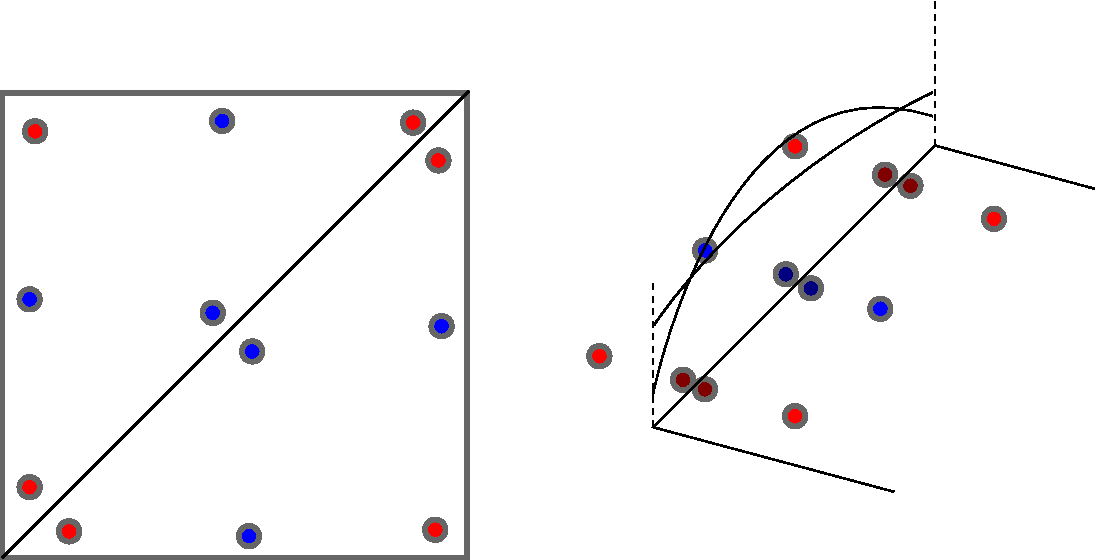
\includegraphics[width=0.65\textwidth]{60_exahype/Ghoddess-dof-layout.pdf}
%  \end{center}
%  \caption{
%   Left: Degree of freedom layout in Ghoddess within a cell.
%   Right: Each face holds additional ``degree of freedoms'' which encode the
%   projection of the cell polynomial onto the face.
%   \label{figure:60_exahype:degree-of-freedom-layout:Ghoddess}
%  }
% \end{figure}
% 
% The Ghoddess solver itself splits up into four computation kernels:
% 
% \begin{enumerate}
%   \item The {\bf projectOntoFace} kernel accepts the $N$ degrees of freedom from
%   the cell and projects the polynomials of the two triangles within the cell
%   onto the faces. It consequently writes $2d \cdot (p+1)^{d-1}$ face DoFs. Once
%   we have traversed the whole mesh, each face ``knows'' its left and right
%   projection.
%   \item The {\bf solveRiemann} kernel takes the $2 \cdot (p+1)^{d-1}$ DoFs on
%   the face, i.e.~the left and right projection, and solves the Riemann problem
%   on the jump. The result is written back into the $2 \cdot (p+1)^{d-1}$ DoFs.
%   In principle, this allows us to have a different outgoing flux for the left
%   and right side of a face.
%   \item The {\bf solveCell} kernel evolves the solution within the triangle
%   pair, i.e.~it evaluates the volumetric integrals of the DG formulation. The
%   name is slightly wrong: Besides the volumetric terms, the kernel also
%   evaluates the face terms arising between the two triangles embedded into the
%   cell. So it is a combination of a cell kernel plus one Riemann solve (in 2d).
%   \item The {\bf projectOntoCell} kernel takes the Riemann solution on the cell
%   faces, i.e.~the output of projectOntoFace, and adds it to the cell solution,
%   i.e.~it adds it to the outcome of solveCell.
% \end{enumerate}
% 
% 
% \noindent
% Ghoddess' vanilla version indeed traverses the mesh four times per time step.
% This makes it easy/easier to debug the code and to analyse the substeps.
% The work of Charrier et al then automatically fuses the traversals and thus
% reduces the memory accesses and homogenises the computational character over the
% mesh sweeps.
% 
% 
% The realisation of the four sweeps relies on blockstructured extension of
% \Peano:
% Though the data is logically not Cartesian or block-structured, we model all
% properties as blocks embedded into the mesh.
% 
% 
% All solvers inherit from \texttt{exahype2.ghoddess.Solver} which is our abstract
% framework.
% Per solver, the Python API will generate one C++ solver class.
% This class has a couple of things to do:
% 
% \begin{enumerate}
%   \item It holds all time stepping data. So it knows, for example, what the
%   minimal time stamp at the moment is.
%   \item It serves as a state machine which decides at any point which kernels
%   are to be executed on particular grid entities.
%   \item It holds the application domain-specific routines such as the actual
%   kernel implementations, refinement criteria or data initialisation.
% \end{enumerate}



\section*{Links and further reading}

\begin{itemize}
  \item The ``official'' ExaHyPE release paper is
{\tiny \begin{verbatim}
@article{Reinarz:2019:ExaHyPE,   
  title = "ExaHyPE: An engine for parallel dynamically adaptive simulations of wave problems",
  journal = "Computer Physics Communications",
  pages = "107251",
  year = "2020",
  issn = "0010-4655",
  doi = "https://doi.org/10.1016/j.cpc.2020.107251",
  url = "http://www.sciencedirect.com/science/article/pii/S001046552030076X",
  author = "Anne Reinarz and Dominic E. Charrier and Michael Bader and Luke Bovard and Michael Dumbser 
    and Kenneth Duru and Francesco Fambri and Alice-Agnes Gabriel and Jean-Matthieu Gallard and 
    Sven Köppel and Lukas Krenz and Leonhard Rannabauer and Luciano Rezzolla and Philipp Samfass and 
    Maurizio Tavelli and Tobias Weinzierl",
  keywords = "Hyperbolic, PDE, ADER-DG, Finite volumes, AMR, MPI, TBB, MPI+X",
}
  \end{verbatim}}
  If you use the software, it would be great if you could cite this one.
\end{itemize}

